\documentclass{article}
\usepackage[T1]{fontenc}
\usepackage{lmodern}
\usepackage{graphicx}
\usepackage{amsmath,amssymb}
\usepackage[a4paper,margin=2cm]{geometry}
\usepackage[absolute,overlay]{textpos}
\setlength{\TPHorizModule}{1mm}
\setlength{\TPVertModule}{1mm}
\usepackage[indonesian]{babel}
\usepackage{hyperref}
\setlength{\emergencystretch}{2em}
\title{14-Algoritma-Elgamal-2026}
\author{pdf\_ppt\_to\_latex}
\date{}

\begin{document}

% --- unit llm 1 ---
% === Halaman 1 (llm) ===

\begin{center}
Bahan kuliah IF4020 Kriptografi

{\huge \textcolor{red}{Algoritma ElGamal}}

\vspace{30mm}

Oleh: Dr. Ir. Rinaldi, M.T

\vspace{10mm}

Program Studi Teknik Informatika\\
Sekolah Teknik Elektro dan Informatika\\
Institut Teknologi Bandung\\
2026
\end{center}

\newpage

% --- unit llm 2 ---
% === Halaman 2 (llm) ===

\section*{Pendahuluan}

\vspace{129.79mm}

\begin{itemize}
    \item Algoritma Elgamal dibuat oleh Taher Elgamal (1985). Pertama kali dikemukakannya di dalam makalah berjudul "A public key cryptosystem and a signature scheme based on discrete logarithms", dimuat di dalam \href{https://ieeexplore.ieee.org/document/1056437}{IEEE Transactions on Information Theory} ( Volume: 31, \href{https://ieeexplore.ieee.org/document/1056437}{Issue: 4}, July 1985)
\end{itemize}

\vspace{10mm}

% deskripsi: Foto profil Taher Elgamal dengan teks 'Taher Elgamal Founder, Securify'
% bbox normalisasi: [0.1130, 0.4880, 0.4920, 0.9060]
\begin{textblock*}{79.59mm}(23.73mm,144.94mm)
\noindent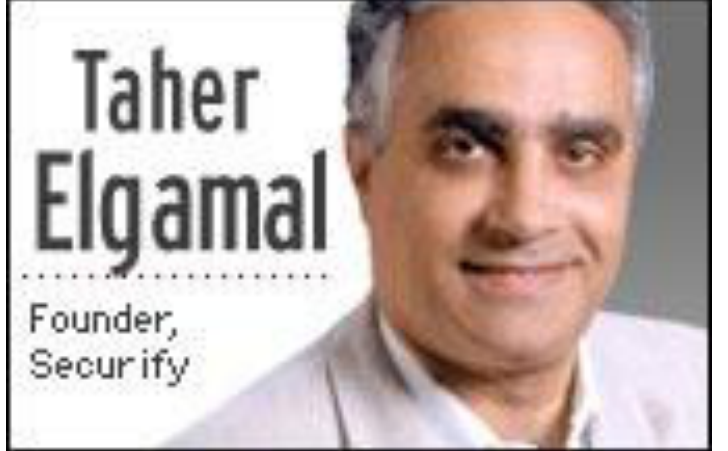
\includegraphics[width=79.59mm,height=124.15mm]{images/llm/page_002_img_01.png}%
\end{textblock*}

% deskripsi: Foto Taher Elgamal saat menerima Lifetime Achievement Award di RSACONFERENCE 2009
% bbox normalisasi: [0.5210, 0.4880, 0.9010, 0.9250]
\begin{textblock*}{79.80mm}(109.41mm,144.94mm)
\noindent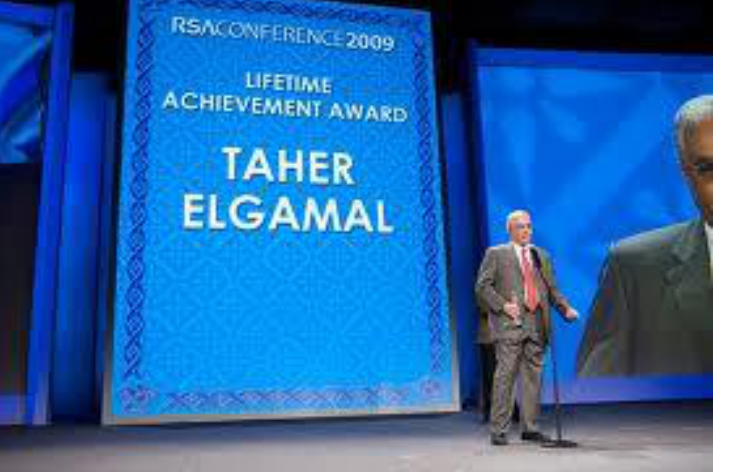
\includegraphics[width=79.80mm,height=129.79mm]{images/llm/page_002_img_02.png}%
\end{textblock*}

\newpage

% --- unit llm 3 ---
% === Halaman 3 (llm) ===

\begin{center}
\textbf{A PUBLIC KEY CRYPTOSYSTEM AND A SIGNATURE SCHEME BASED ON DISCRETE LOGARITHMS}\
\vspace{1em}
Taher ElGamal$^*$\
\vspace{1em}
Hewlett-Packard Labs\\
1501 Page Mill Rd.\\
Palo Alto CA 94301
\end{center}

\textbf{ABSTRACT}

A new signature scheme is proposed together with an implementation of the Diffie - Hellman key distribution scheme that achieves a public key cryptosystem. The security of both systems relies on the difficulty of computing discrete logarithms over finite fields.

\textbf{1. INTRODUCTION}

In 1976, Diffie and Hellman [3] introduced the concept of public key cryptography. Since then, several attempts have been made to find practical public key systems (see for example [6,7,9]) depending on the difficulty of solving some problems. For example, the RSA system [9] depends on the difficulty of factoring large integers. This paper presents systems that rely on the difficulty of computing logarithms over finite fields.

Section 2 shows a way to implement the public key distribution scheme introduced by Diffie and Hellman [3] to encrypt and decrypt messages. The security of this system is equivalent to that of the distribution scheme. Section 3 introduces a new digital signature

\newpage

% --- unit llm 4 ---
% === Halaman 4 (llm) ===

\begin{itemize}
    \item Keamanan algoritma ini terletak pada sulitnya menghitung logaritma diskrit.
    \item \textit{Persoalan logaritma diskrit}: Jika $p$ adalah bilangan prima dan $g$ dan $y$ adalah sembarang bilangan bulat, carilah $x$ sedemikian sehingga
    \[ g^x \equiv y \pmod{p} \]
\end{itemize}

Contoh: $7^x \equiv 15 \pmod{41}$, berapakah nilai $x$?

\begin{itemize}
    \item Sebelum membahas algoritma ElGamal lebih lanjut, maka kita perlu memahami terlebih dahulu tentang logaritma diskrit dan akar primitif dari sebuah bilangan prima.
\end{itemize}

\newpage

% --- unit llm 5 ---
% === Halaman 5 (llm) ===

\section*{Akar Primitif dan Logaritma Diskrit}

\begin{itemize}
    \item Jika $n$ adalah bilangan bulat, maka $a$ disebut \textbf{akar primitif} dari $n$ jika perpangkatan
    \[ a, a^2, ..., a^{\phi(n)} \quad (\text{dalam sebuah modulus } n) \]
    menghasilkan nilai yang berbeda dan semuanya relatif prima dengan $n$.
    
    \item Secara khusus, jika $p$ adalah bilangan prima, maka $a$ disebut akar primitif dari $p$ jika perpangkatan
    \[ a, a^2, ..., a^{p-1} \quad (\text{dalam modulus } p) \]
    menghasilkan nilai-nilai yang berbeda \\
    (ingatlah dari fungsi \textit{toitient} Euler, bahwa jika $p$ prima maka $\phi(p) = p - 1$)
\end{itemize}

\newpage

% --- unit llm 6 ---
% === Halaman 6 (llm) ===

\begin{itemize}
  \item Sebagai contoh, misalkan $p = 7$, maka $a = 3$ adalah akar primitif dari 7 karena
  \[ 
  \begin{aligned}
  3^1 \pmod 7 &= 3; & 3^2 \pmod 7 &= 2; & 3^3 \pmod 7 &= 6 \\
  3^4 \pmod 7 &= 4; & 3^5 \pmod 7 &= 5; & 3^6 \pmod 7 &= 1
  \end{aligned}
  \]
  \item Jadi, semua perpangkatan dari 3 menghasilkan nilai-nilai yang berbeda $(3, 2, 6, 4, 5, 1)$, semua bilangan di dalam modulus 7 terjadi satu kali.
  \item Perpangkatan berikutnya, $3^7 \pmod 7, 3^8 \pmod 7, \dots,$ akan kembali berulang menghasilkan nilai-nilai tersebut. Panjang satu siklus tidak lebih dari $7 - 1 = 6$.
  \item Secara umum, untuk $p$ bilangan prima, maka panjang siklus tidak lebih dari $p - 1$.
\end{itemize}

\newpage

% --- unit llm 7 ---
% === Halaman 7 (llm) ===

\begin{itemize}
    \item Perhatikan bahwa $a = 2$ bukan akar primitif dari 7 karena
    
    \[
    \begin{aligned}
    2^1 \pmod{7} &= 2; & 2^2 \pmod{7} &= 4; & 2^3 \pmod{7} &= 1 \\
    2^4 \pmod{7} &= 2; & 2^5 \pmod{7} &= 4; & 2^6 \pmod{7} &= 1
    \end{aligned}
    \]
    
    \item Nilai-nilai yang dihasilkan dari $2^1, 2^2, \dots, 2^6$ tidak semuanya berbeda dan tidak mencakup semua nilai di dalam modulus 7.
    
    \item Untuk menemukan semua akar primitif dari $p$, kita harus mencoba semua bilangan bulat dari $2, 3, \dots$
\end{itemize}

\newpage

% --- unit llm 8 ---
% === Halaman 8 (llm) ===

\begin{itemize}
  \item Jika $a$ adalah akar primitif dari bilangan prima $p$, maka untuk bilangan bulat $b$ kita dapat menemukan pangkat $x$ sedemikian sehingga
  \[ b \equiv a^x \pmod{p}, \quad 0 \le x \le (p-1) \]
  \item Pangkat $x$ disebut \textbf{logaritma diskrit} dari $b$ untuk basis $a \pmod{p}$.
  \item Dalam \textbf{persoalan logaritma diskrit}, diberikan $b \equiv a^x \pmod{p}$, carilah $x$ yang memenuhi kekongruenan tersebut.
  \item Sebagai contoh, 7 adalah akar primitif dari bilangan prima $p = 41$. Maka, carilah $x$ sedemikian sehingga $15 \equiv 7^x \pmod{41}$, jawabannya adalah 3 karena
  \[ 7^3 = 343 \equiv 15 \pmod{41} \]
\end{itemize}

\newpage

% --- unit llm 9 ---
% === Halaman 9 (llm) ===

Properti algoritma ElGamal:
\begin{enumerate}
  \item Bilangan prima, $p$ \hfill (tidak rahasia)
  \item Bilangan acak, $g$ ($g < p, g$ adalah akar primitif dari $p$) \hfill (tidak rahasia)
  \item Bilangan acak, $x$ ($2 \le x \le p - 2$) \hfill (rahasia, \textcolor{red}{kunci privat})
  \item $y = g^x \pmod{p}$ \hfill (tidak rahasia, \textcolor{red}{kunci publik})
  \item $m$ (plainteks) \hfill (rahasia)
  \item $a$ dan $b$ (cipherteks) \hfill (tidak rahasia)
\end{enumerate}

\newpage

% --- unit llm 10 ---
% === Halaman 10 (llm) ===

\section*{Prosedur Pembangkitan Kunci}

\begin{enumerate}
    \item Pilih sembarang bilangan prima $p$ ($p$ dapat di-share di antara anggota kelompok)
    \item Pilih dua buah bilangan acak, $g$ dan $x$, dengan syarat $g < p$, $g$ akar primitif dari $p$, dan $2 \le x \le p - 2$
    \item Hitung $y = g^x \pmod{p}$ \hfill (1)
\end{enumerate}

\noindent Hasil dari algoritma ini:
\begin{itemize}
    \item Kunci publik: tripel $(y, g, p)$
    \item Kunci privat: pasangan $(x, p)$
\end{itemize}

\newpage

% --- unit llm 11 ---
% === Halaman 11 (llm) ===

\section*{Prosedur Enkripsi}

\begin{enumerate}
    \item \textbf{Preprocessing}: Jika plainteks $m$ berukuran besar, pecah plainteks menjadi blok-blok $m_1, m_2, \dots,$ (nilai setiap blok harus berada di dalam selang $[0, p - 1]$.
    \item Pilih bilangan acak $k$, yang dalam hal ini $1 \le k \le p - 2$.
    \item Setiap blok $m$ dienkripsi dengan rumus
    \begin{align}
        a &= g^k \pmod{p} \tag{2} \\
        b &= y^k m \pmod{p} \tag{3}
    \end{align}
    Pasangan $(a, b)$ adalah cipherteks untuk blok pesan $m$. Jadi, ukuran cipherteks adalah dua kali ukuran plainteksnya.
\end{enumerate}

\newpage

% --- unit llm 12 ---
% === Halaman 12 (llm) ===

\section*{Prosedur Dekripsi}

\begin{enumerate}
    \item Gunakan kunci privat $x$ untuk menghitung $(a^x)^{-1} = a^{p-1-x} \pmod{p}$
    \item Hitung plainteks $m$ dengan persamaan:
    \[ m = b/a^x \pmod{p} = b(a^x)^{-1} \pmod{p} \]

\newpage

% --- unit llm 13 ---
% === Halaman 13 (llm) ===

Bukti bahwa pesan $m$ dapat diungkap kembali dari pasangan cipherteks $a$ dan $b$:

Dari persamaan (2): $a = g^k \pmod p \rightarrow g^k \equiv a \pmod p$

Pangkatkan kedua ruas dengan $x$ : $g^{xk} \equiv a^x \pmod p$

Dari persamaan (3): $b = y^k m \pmod p \rightarrow y^k m \equiv b \pmod p$

Dari persamaan (1): $y = g^x \pmod p \rightarrow g^x \equiv y \pmod p$,

maka

\begin{align*}
 b/a^x &\equiv y^k m / a^x \pmod p \\
 &\equiv g^{xk} m / g^{xk} \pmod p \\
 &\equiv m \pmod p
\end{align*}

yang berarti bahwa plainteks $m$ dapat diungkap kembali dari cipherteks $a$ dan $b$.

\newpage

% --- unit llm 14 ---
% === Halaman 14 (llm) ===

\textbf{Contoh 1:} Bob membangkitkan kunci publik dan kunci privatnya. Alice akan mengenkripsi pesan dengan menggunakan kunci publik Bob.

\textbf{(a) Pembangkitan kunci} (Oleh Bob)

\textcolor{red}{syarat $g < p, g$ akar primitif dari 2357 dan $1 \le x \le p - 2$}

Misal $p = 2357, g = 2,$ dan $x = 1751$.

Hitung: $y = g^x \pmod p = 2^{1751} \pmod{2353} = 1185$

Hasil: Kunci publik: $(y = 1185, g = 2, p = 2357)$

Kunci privat: $(x = 1751, p = 2357)$.

Bob memberitahu kunci publik ini kepada Alice

\vspace{10mm}

\textbf{(b) Enkripsi} (Oleh Alice)

Misalkan pesan $m = 2035$ (nilai $m$ masih berada di dalam selang $[0, 2357 - 1])$.

Alice memilih bilangan acak $k = 1520$ (nilai $k$ berada di dalam selang $[0, 2357 - 1])$.

\newpage

% --- unit llm 15 ---
% === Halaman 15 (llm) ===

Alice melakukan enkripsi dengan kunci public Bob ($y = 1185, g = 2, p = 2357$):
\[ a = g^k \pmod p = 2^{1520} \pmod{2357} = 1430 \]
\[ b = y^k m \pmod p = 1185^{1520} \cdot 2035 \pmod{2357} = 697 \]

Jadi, cipherteks yang dihasilkan adalah $(1430, 697)$.\nAlice mengirim cipherteks ini kepada Bob.

\textbf{(c) Dekripsi (Oleh Bob)}

Bob melakukan dekripsi dengan kunci privatnya ($x = 1751, p = 2357$):
\[ (a^x)^{-1} = a^{p-1-x} \pmod p = 1430^{2357-1-1751} \pmod{2357} = 1430^{605} \pmod{2357} = 872 \]
\[ m = b/a^x \pmod p = b \cdot (a^x)^{-1} \pmod p = 697 \cdot 872 \pmod{2357} = 2035 \]

Bob mendapatkan kembali plainteks $m = 2035$ yang dikirim oleh Alice.

\newpage

% --- unit llm 16 ---
% === Halaman 16 (llm) ===

\textbf{Contoh 2:} Alice membangkitkan pasangan kuncinya. Bob akan mengirim pesan dengan menggunakan kunci publik Alice.

\textbf{(a) Pembangkitan kunci (oleh Alice)}

Alice memilih bilangan prima $p = 2273$, akar primitif dari $p$ yaitu $g = 3$, dan $x = 243$.

Alice kemudian menghitung:
\[ y = g^x \pmod{p} = 3^{243} \pmod{2273} = 461 \]

Jadi,

\begin{itemize}
    \item kunci privat Alice: $(x = 243, p = 2273)$
    \item kunci publik Alice: $(y = 461, g = 3, p = 2273)$.
\end{itemize}

\newpage

% --- unit llm 17 ---
% === Halaman 17 (llm) ===

\textbf{(b) Enkripsi (oleh Bob)}\newline
Misalkan Bob ingin mengirim plainteks 'HALO' kepada Alice.

Misalkan A = 00, B = 01, ..., Z = 25, maka pesan $m$ dikodekan ke dalam \textit{integer} adalah
\[ m = 07001114 \]

Bob memecah $m$ menjadi blok yang lebih kecil, misalkan $m$ dipecah menjadi blok-blok sepanjang 4 angka:
\[ m_1 = 0700 \quad \text{dan} \quad m_2 = 1114 \]

Nilai-nilai $m_i$ ini masih terletak di dalam selang $[0, 2273 - 1]$ agar transformasi menjadi satu-ke-satu.

\newpage

% --- unit llm 18 ---
% === Halaman 18 (llm) ===

(i) Enkripsi $m_1 = 0700$

Bob memilih bilangan acak $k = 1463$ (nilai $k$ masih berada di dalam selang $[0, 2273 - 1]$).

Bob mengenkripsi pesan dengan menggunakan kunci publik Alice ($y = 461, g = 3, p = 2273$):

\[ a = g^k \bmod p = 3^{1463} \bmod 2273 = 1439 \]
\[ b = y^k m_1 \bmod p = 461^{1463} \cdot 700 \bmod 2273 = 74 \]

Jadi, cipherteks yang dihasilkan untuk $m_1$ adalah $\mathbf{c_1 = (1439, 74)}$.

\vspace{10mm}

(ii) Enkripsi $m_2 = 1114$

Bob memilih bilangan acak $k = 2001$ (nilai $k$ masih berada di dalam selang $[0, 2273 - 1]$).

Bob mengenkripsi pesan dengan menggunakan kunci publik Alice ($y = 461, g = 3, p = 2273$):

\[ a = g^k \bmod p = 3^{2001} \bmod 2273 = 1220 \]
\[ b = y^k m_2 \bmod p = 461^{2001} \cdot 1114 \bmod 2273 = 1682 \]

Jadi, cipherteks yang dihasilkan untuk $m_2$ adalah $\mathbf{c_2 = (1220, 1682)}$.

Bob mengirim cipherteks $(1439, 74)$ dan $(1220, 1682)$ kepada Alice.

\newpage

% --- unit llm 19 ---
% === Halaman 19 (llm) ===

\textbf{(c) Dekripsi (oleh Alice)}

Alice mendekripsi cipherteks dari Bob dengan kunci privatnya ($x = 243$, $p = 2273$):

\begin{enumerate}
  \item[(i)] Dekripsi $c_1 = (1439, 74)$
  \[ (a^x)^{-1} = a^{p-1-x} \pmod p = 1439^{2273-1-243} \pmod{2273} = 1439^{2029} \pmod{2273} = 1791 \]
  \[ m_1 = b/a^x \pmod p = b(a^x)^{-1} \pmod p = 74 \cdot 1791 \pmod{2273} = 700 = \text{\color{red}0700} \]
  \item[(ii)] Dekripsi $c_2 = (1220, 1682)$
  \[ (a^x)^{-1} = a^{p-1-x} \pmod p = 1220^{2029} \pmod{2273} = 1125 \]
  \[ m_2 = b/a^x \pmod p = 1682(a^x)^{-1} \pmod p = 1682 \cdot 1125 \pmod{2273} = \text{\color{red}1114} \]
\end{enumerate}

Plainteks yang didekripsi adalah $m_1 m_2 = 07001114$, yang kalau dikodekan menjadi teks adalah empat digit adalah "HALO", sama dengan plainteks yang dikirim oleh Bob.

\newpage

% --- unit llm 20 ---
% === Halaman 20 (llm) ===

\vspace{231.66mm}

\begin{itemize}
    \item Demo online enkripsi ElGamal: \url{https://www.debjitbiswas.com/elgamal/}
\end{itemize}

\vspace{10mm}

% deskripsi: Screenshot dari ElGamal Encryption Playground yang menunjukkan proses enkripsi dan dekripsi antara Alice dan Bob, termasuk input prime p, generator g, private key, serta rumus matematika untuk perhitungan h, c1, c2, s, dan m.
% bbox normalisasi: [0.0900, 0.1300, 0.9300, 0.9100]
\begin{textblock*}{176.40mm}(18.90mm,38.61mm)
\noindent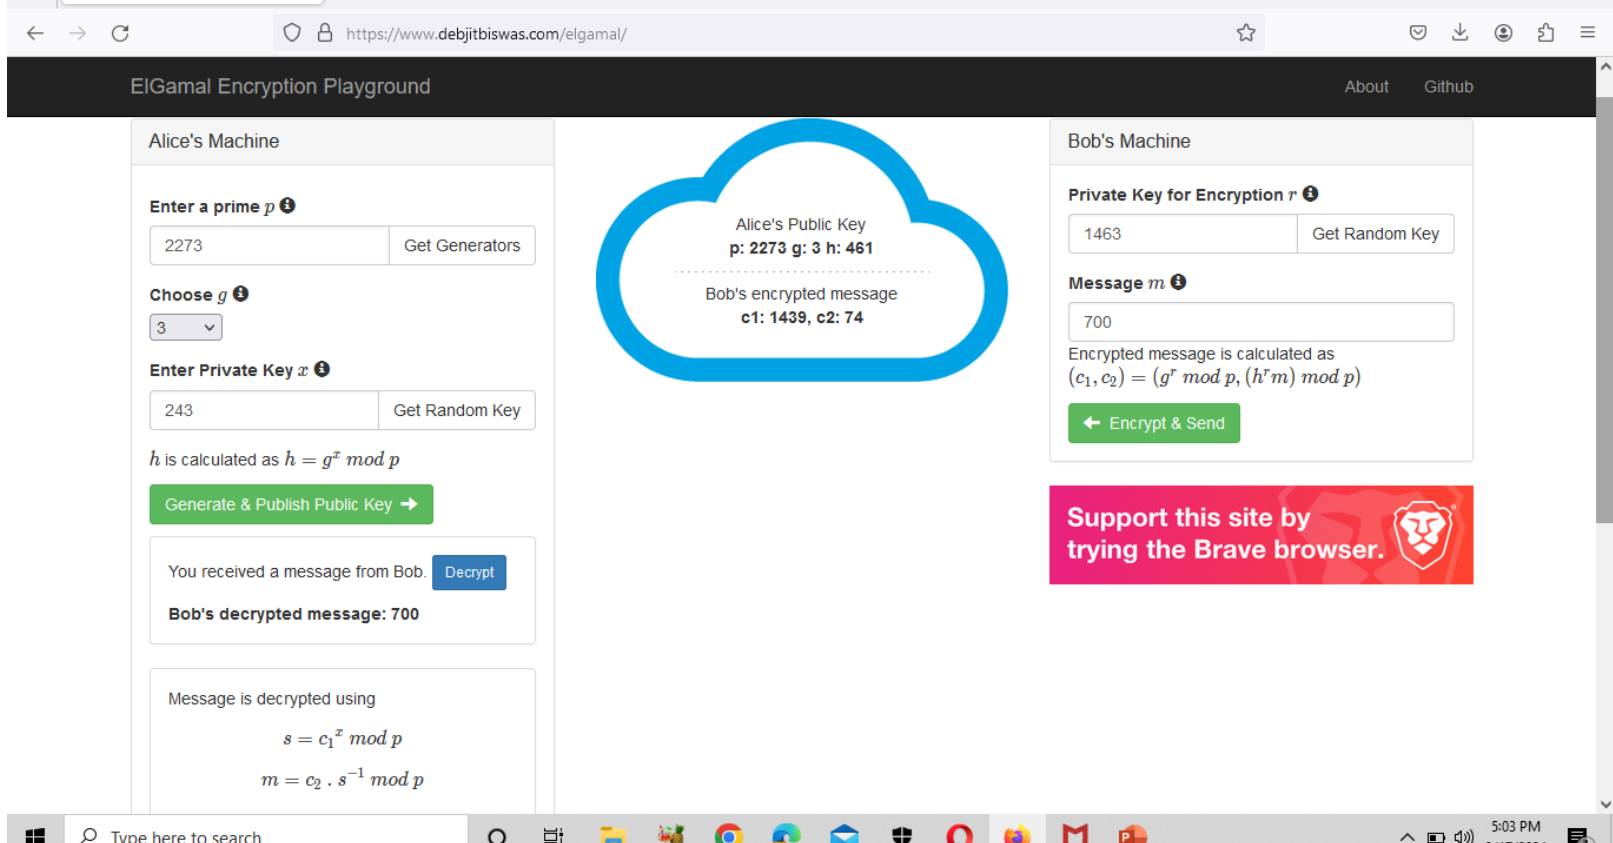
\includegraphics[width=176.40mm,height=231.66mm]{images/llm/page_020_img_01.png}%
\end{textblock*}

\end{document}
